\documentclass[tikz,border=10pt]{standalone}
\usepackage{tikz}
\usetikzlibrary{positioning, arrows.meta}

\begin{document}
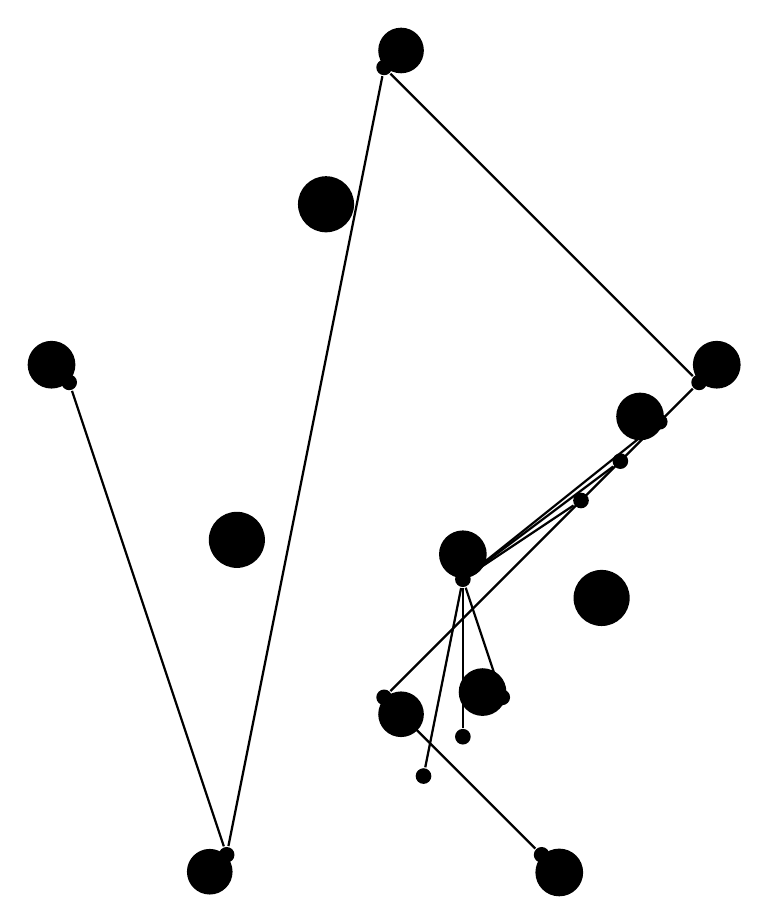
\begin{tikzpicture}[
    node distance=2cm and 2cm,
    >=Latex,
    every node/.style={circle, inner sep=2pt, fill=black},
    line width=0.8pt
]

% Define main nodes
\node (u1) at (4,0) {};
\node (v1) at (0,-4) {};
\node (u2) at (2,-6) {};
\node (v2) at (-2,-6) {};
\node (u3) at (-4,0) {};
\node (v3) at (0,4) {};

% Connect main nodes
\draw (u1) -- (v1) -- (u2) -- cycle;
\draw (u3) -- (v2) -- (v3) -- cycle;
\draw (u1) -- (v3);

% Label main nodes
\node[above right] at (u1) {$u_1$};
\node[below right] at (v1) {$v_1$};
\node[below right] at (u2) {$u_2$};
\node[below left] at (v2) {$v_2$};
\node[above left] at (u3) {$u_3$};
\node[above right] at (v3) {$v_3$};

% Define x1 nodes
\node (x11) at (3.5, -0.5) {};
\node (x12) at (3, -1) {};
\node (x13) at (2.5, -1.5) {};

% Label x1 region
\node[above] at (3.25, -0.75) {$x_1$};

% Define x2 nodes
\node (x21) at (1.5, -4) {};
\node (x22) at (1, -4.5) {};
\node (x23) at (0.5, -5) {};

% Label x2 region
\node[above] at (1.25, -4.25) {$x_2$};

% Define x3 node
\node (x3) at (1, -2.5) {};

% Label x3 region
\node[above] at (1, -2.5) {$x_3$};

% Connect x1 nodes to x3
\foreach \i in {1,2,3}{
    \draw (x1\i) -- (x3);
}

% Connect x2 nodes to x3
\foreach \i in {1,2,3}{
    \draw (x2\i) -- (x3);
}

% Draw regions R1, R2, R3
\node[above right] at (2.5, -3) {$R_1$};
\node[left] at (-1.5, -2) {$R_2$};
\node[above right] at (-1, 2) {$R_3$};

\end{tikzpicture}
\end{document}